\documentclass[sigconf,review, anonymous]{acmart}
%\acmConference[ESEC/FSE 2019]{The 27th ACM Joint European Software Engineering
% Conference and Symposium on the Foundations of Software Engineering}{26--30 August, 2019}{Tallinn, Estonia}

\usepackage[norelsize,linesnumbered,ruled,vlined]{algorithm2e}

\pagestyle{plain}

%\usepackage[latin1]{inputenc}
\usepackage{graphicx}
%\usepackage{algorithm}
\usepackage{algorithmic}
\usepackage{multirow}
\usepackage{longtable}
\usepackage{rotating}
\usepackage{enumerate}
%\usepackage{slashbox}
%\usepackage{amsthm}
\usepackage{amsmath}
\usepackage{xcolor}
\usepackage{epstopdf}
\usepackage{subfigure}
\usepackage{listings}
\usepackage{xcolor}
\usepackage{url}
\usepackage{caption}
\usepackage{hyperref}
\usepackage{slashbox,multirow}
%\usepackage{flushend}
%\reference alignment
\definecolor{keywordcolor}{rgb}{0,0,1.0}
\definecolor{lightgreen}{rgb}{0,0.8,0}
\definecolor{webgreen}{rgb}{0,0.5,0}

\newcommand{\hytt}[1]{\texttt{\hyphenchar\font=\defaulthyphenchar #1}}
\newtheorem{definition}{Definition}
\newtheorem{pattern}{Anti-pattern}
%\renewcommand{\algorithmicrequire}{\textbf{Input:}}
%\renewcommand{\algorithmicensure}{\textbf{Output:}}

% Copyright
%\setcopyright{none}
%\setcopyright{acmcopyright}
%\setcopyright{acmlicensed}
%\setcopyright{rightsretained}
%\setcopyright{usgov}
%\setcopyright{usgovmixed}
%\setcopyright{cagov}
%\setcopyright{cagovmixed}

\lstset{
  language=Java,
  alsolanguage= XML,
  tabsize=4, %
  frame=, %把代码用带有阴影的框圈起来
  %rulesepcolor=\color{red!20!green!20!blue!20},%代码块边框为淡青色
  keywordstyle=\color{red!20!green!20!blue!20}, %代码关键字的颜色为蓝色,粗体
  showstringspaces=false,%不显示代码字符串中间的空格标记
  stringstyle=\ttfamily, % 代码字符串的特殊格式
  keepspaces=true, %
  breakindent=22pt, %
  %frame=single,
  numbers=left,%左侧显示行号 往左靠,还可以为right,或none,即不加行号
  stepnumber=1,%若设置为2,则显示行号为1,3,5,即stepnumber为公差,默认stepnumber=1
  %numberstyle=\tiny, %行号字体用小号
  numberstyle={\color[RGB]{0,204,0}\tiny} ,%设置行号的大小,大小有tiny,scriptsize,footnotesize,small,normalsize,large等
  numbersep=8pt,  %设置行号与代码的距离,默认是5pt
  commentstyle={\color{green}\tiny},%浅灰色的注释
  basicstyle=\footnotesize, % 这句设置代码的大小
  showspaces=false, %
  flexiblecolumns=true, %
  breaklines=true, %对过长的代码自动换行
  breakautoindent=true,%
  breakindent=4em, %
  %aboveskip=1em, %代码块边框
  tabsize=2,
  showstringspaces=false, %不显示字符串中的空格
  fontadjust,
  framextopmargin=2pt,framexbottommargin=2pt,abovecaptionskip=-3pt,belowcaptionskip=3pt,
  xleftmargin=1em,xrightmargin=1em, % 设定listing左右的空白
}

\lstset{language=[AspectJ]Java,
basicstyle=\footnotesize,
keywordstyle=\color{keywordcolor}, %\underbar,
identifierstyle=,
commentstyle=\color{lightgreen} \textit,
stringstyle=\ttfamily,
showstringspaces=false,
captionpos=b
}


% DOI
% \acmDOI{10.475/123_4}
%
% % ISBN
% \acmISBN{123-4567-24-567/08/06}
%
% %Conference
% \acmConference[]{ESEC/FSE'19}{26--30 August, 2019}{Tallinn, Estonia}
% \acmYear{2018}
% \copyrightyear{2018}
%
%
% %\acmArticle{4}
% \acmPrice{15.00}


% These commands are optional
%\acmBooktitle{Transactions of the ACM Woodstock conference}
%\editor{Jennifer B. Sartor}
%\editor{Theo D'Hondt}
%\editor{Wolfgang De Meuter}

\setcopyright{none}
\begin{document}
\title{ServDroid: Detecting Service Usage Inefficiencies in\\  Android Applications}
%\titlenote{Produces the permission block, and copyright information}
%\subtitle{Extended Abstract}
%\subtitlenote{The full version of the author's guide is available as \texttt{acmart.pdf} document}

\iffalse
\author{Wei Song, Jing Zhang}
%\authornote{Dr.~Trovato insisted his name be first.}
\orcid{0000-0002-4324-3382}
\affiliation{%
  \institution{School of Computer Science and Engineering\\Nanjing University of Science and Technology}
  \streetaddress{Xiaolingwei 200}
  \city{Nanjing}
  %\state{Ohio}
  \country{China}
  \postcode{210094}
}
\email{wsong@njust.edu.cn}

\author{Jeff Huang}
%\authornote{This author is the one who did all the really hard work.}
\affiliation{%
  \institution{Parasol Laboratory\\Texas A\&M University}
  %\streetaddress{1 Th{\o}rv{\"a}ld Circle}
  \city{College Station, TX}
  \country{USA}}
\email{jeff@cse.tamu.edu}

% The default list of authors is too long for headers.
\renewcommand{\shortauthors}{}

\fi

\begin{abstract}
Services in Android applications are frequently-used components for performing
time-consuming operations in the background. While services play a crucial role
in the app performance, our study shows that service usages in practice are not
as efficient as expected, e.g., they tend to cause unnecessary resource occupation
and/or energy consumption.
Moreover, as service usage inefficiencies do not manifest
with immediate app failures, e.g., crashes, existing testing-based approaches
fall short in finding them.
In this paper, we identify four anti-patterns of such service usage
inefficiency bugs, including premature create, late destroy, premature destroy,
and service leak, and present a static analysis technique, \textsf{ServDroid},
to automatically and effectively detect them based on the anti-patterns.
We have applied \textsf{ServDroid} to a large collection of popular real-world
Android apps and, surprisingly, we find that service usage inefficiencies are
pervalent and can severely impact apps' energy consumption.
\end{abstract}

%
% The code below should be generated by the tool at
% http://dl.acm.org/ccs.cfm
% Please copy and paste the code instead of the example below.
%
% \begin{CCSXML}
% <ccs2012>
% <concept>
% <concept_id>10011007.10011074.10011099.10011102</concept_id>
% <concept_desc>Software and its engineering~Software defect analysis</concept_desc>
% <concept_significance>500</concept_significance>
% </concept>
% <concept>
% <concept_id>10011007.10011074.10011099.10011102.10011103</concept_id>
% <concept_desc>Software and its engineering~Software testing and debugging</concept_desc>
% <concept_significance>500</concept_significance>
% </concept>
% </ccs2012>
% \end{CCSXML}
%
% \ccsdesc[500]{Software and its engineering~Software defect analysis}
% \ccsdesc[500]{Software and its engineering~Software testing and debugging}
%
% \keywords{Android app, background service, usage inefficiency, service leak, static analysis}


\maketitle

\section{Introduction}
Mobile is eating the world.
%Millions of mobile apps are available on Google Play
%and Apple App stores, and many apps have millions or even billions of downloads.
The improvement of computation and memory capacity of mobile devices allows
developers to design increasingly powerful and complex apps. On the other hand,
more complex apps usually involve more bugs and vulnerabilities, which
significantly impact the release and adoption of the apps.
Thus, the quality of mobile apps receives much and increasing
attention~\cite{ReavesBGABCDHKS16,AnandNHY12,MachiryTN13,ChoiNS13,LiuXC14,BanerjeeC0R14,LiuXCL14,HechtBRMD15,BehrouzSBM16,MirzaeiGBSM16,SuMCWYYPLS17,FanSCMLXPS18}.

Testing is an effective means to find bugs and to help assure the quality of
apps.
Since Android is popular, many testing approaches have
been developed for Android apps. Nonetheless, they mostly focus on GUI testing
of foreground activities~\cite{monkey,AnandNHY12,MachiryTN13,ChoiNS13,MirzaeiGBSM16,BaekB16,SuMCWYYPLS17,SongQH17},
whereas background services have received few research
attention~\cite{ZhangLLC17,ma2018}. Services are Android components that perform
long-running tasks involving few or no user interactions, e.g., file I/O, music
playing, or network transactions~\cite{Androidservice}. A service executes on
the main thread of the calling component's process, and thus a new thread is
often created to perform the long-running operations. Services in Android fall
into two categories: system services and app services.
According to how they are used in the code, app services can
be further divided into three types:
\textit{started services}, \textit{bound services} and \textit{hybrid services}.
% kinds: local services and remote services. Local services are defined by the app itself whereas remote services are from other apps running on the same device.

Although app services usually do not have a user interface, they can keep running
even when the device screen is shut down. As a consequence, if an app involves
service-related bugs, not only the functionalities of the app but its
performance (e.g., resource utilization and energy consumption) can be affected.
In this paper, we focus on app services usage inefficiencies (a type of non-functional bug) that do not immediately lead to app crashes, but
have a significant impact on the performance of the app.
%This problem has received little attention~\cite{ZhangLLC17} in the literature.
Since such bugs do not cause app crashes, existing testing methods do
not work well in detecting them.
Although there exists work on non-functional testing (mainly energy testing) of
apps~\cite{LiuXC14,BanerjeeC0R14,LiuXCL14,BehrouzSBM16,JabbarvandM17},
non-functional testing is generally more expensive and more labour-intensive than functional
testing~\cite{BehrouzSBM16}, because its oracle is usually based on performance
indicators.

%Therefore, a large proportion of app energy consumption is caused by background services~\cite{}.

To address this problem, instead of using testing, we first propose four
anti-patterns to facilitate the analysis of service usage
inefficiency bugs. These anti-patterns are all defined based on the lifecycle
of services~\cite{Androidservice} and are distilled from our manual analysis
of real-world Android apps. The anti-patterns are described below:
\begin{itemize}
  \item {\bf Premature create} refers to the situation that a
service is created too early before it is used. Hence, the service is in
an idle state beginning from its creation to its real use, occupying unnecessary
memory and consuming unnecessary energy.
\item  {\bf Late destroy} refers to the situation
that a service is destroyed too late after its use. Similarly, the service is in
an idle state beginning from the end of its final use to the moment it is destroyed.
\item {\bf Premature destroy} refers to the situation that a service is initiated by a
component (caller) but it is destroyed before another component begins to use
it. Consequently, the service should be created again to fulfil the new request.
\item {\bf Service leak} refers to the situation that a service is never destroyed
after its use, not even when the app which initiated the service terminates.
\end{itemize}

% We observe from real-world apps that these four kinds of efficiency bugs are
% common.
For each of the four service usage anti-patterns, we then propose a scalable
static analysis to automatically detect its instances (concrete efficiency
bugs matching the anti-pattern) in apps.
% The analysis is based on
% \textsf{Soot}~\cite{sootpaper}\footnote{https://github.com/Sable/soot}, a
% framework for transforming and analyzing Java and Android applications.
Our approach takes an app (APK file) as input and performs a context-insensitive
inter-procedural control flow analysis based on Soot~\cite{sootpaper}. It uses
dominator analysis and successor analysis to find the service usage inefficiency
bugs, and also locate the components (callers) that
initiate the services to facilitate debugging.

We implemented our approach in an open-source tool \textsf{ServDroid}. The tool
is written in Java and is publicly available (links are omitted due to double-blind review).
To investigate service usage in real-world apps, we
conducted an empirical analysis on 1,000 Android apps
downloaded from Google Play (accessed in Dec 2018) by applying \textsf{ServDroid} on them.
Our study shows that
service usage inefficiency bugs are surprisingly pervasive in these real-world
apps: 825 (82.5\%) apps involve at least one kind of service usage inefficiency
bug; each app has on average 4.43 service usage inefficiency bugs.
Moreover, our measurement with \textsf{Trepn Profiler}\footnote{https://developer.qualcomm.com/software/trepn-power-profiler} on 38 apps shows that by fixing these bugs an
app can save on average 87.14 Joule of battery in 15 minutes (as much as 15.94\%
energy reduction).
Our empirical study shows that service usage inefficiencies are severe in practice.

%The identified bugs are validated through manual analysis or real phone testing, and some of the bugs are confirmed by developers. Our study takes the first step to address these problems, which can inspire the follow-up research on debugging and repairing such bugs.

In summary, the key contributions of this paper are:
\begin{enumerate}
\item According to the service lifecycle and our manual analysis of real-world apps, we propose four novel service usage
anti-patterns that may lead to unnecessary resource occupation and energy
consumption.
%To our best knowledge, our work is among the first to detect service usage inefficiencies in mobile apps.
\item Based on the anti-patterns, we present a static analysis approach and an
open-source tool, \textsf{ServDroid}, to efficiently detect service usage
inefficiency bugs and also help debug them. The precision and recall of
\textsf{ServDroid} on the top 45 most popular free Android apps listed on
Wikipedia~\footnote{https://en.wikipedia.org/wiki/List\_of\_most\_downloaded\_Android\_applica\\tions
(accessed in Jan 2018)} are 100\% based on our manual study.
\item We conduct an empirical study on 1,000 real-world Android apps, the
results of which demonstrate that the service usage inefficiencies are pervasive
in practice. The experiment on the 45 apps show that service usage inefficiencies indeed have a significant negative impact on energy consumption.
\end{enumerate}

The rest of the paper is organized as follows. Section~\ref{background} gives an
introduction to the three types of app services.
Section~\ref{antipatterns} formulates the four anti-patterns that lead to
service usage inefficiency bugs.
Section~\ref{approach} presents our static analysis for detecting instances
of such anti-patterns.
Section~\ref{evaluation} reports the results of our empirical study.
Section~\ref{relatedwork} reviews related work, and
Section~\ref{conclusion} concludes the paper.

\section{Background}\label{background}
Along with \textit{activities} (user interfaces),
\textit{broadcast receivers} (mailboxes for broadcast), and \textit{content providers} (local database servers), services (background tasks) are fundamental components in Android apps. To ease the understanding of service usage anti-patterns, we introduce the lifecycle of app services and how they are used~\cite{Androidservice}.

To define an app service, one should extends the \hytt{Service} class provided
by Android, and overwrite the corresponding methods of \hytt{Service}, e.g.,
\hytt{onStartCommand(Intent, int, int)}, \hytt{onBind()}, etc. A service is
started in the app by an asynchronous message object which is  referred to as
\textit{intent}. Accordingly, a service declared by a \hytt{$<$service$>$} tag
in the AndroidManifest XML file of the app must have the
\hytt{$<$intent-filter$>$} attribute, which indicates the intents that can start
it. The attribute \hytt{$<$exported$>$} indicates that components from other
apps can invoke or interact with it. The attribute \hytt{$<$isolatedProcess$>$}
indicates whether the service is executed in an isolated process. Services can
be used in three manners, corresponding to three types of app services:
\textit{started service}, \textit{bound service}, and \textit{hybrid service}.

\begin{figure}
  \centering
  \subfigure[]{
    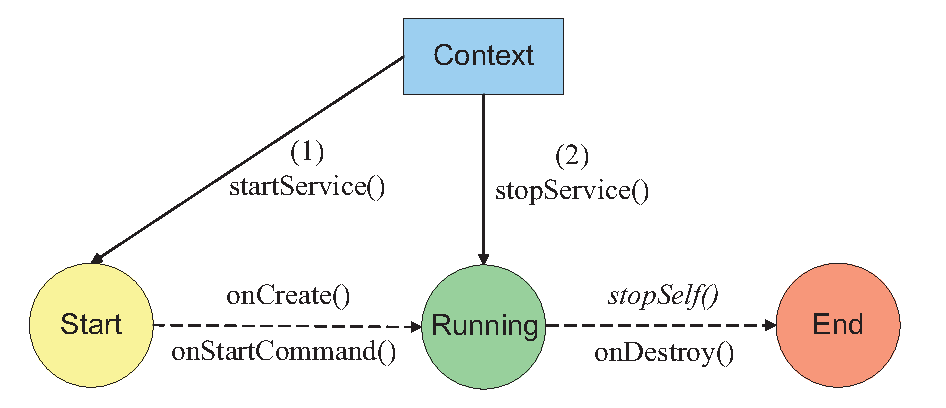
\includegraphics[scale=0.48]{started.eps}}
  \subfigure[]{
    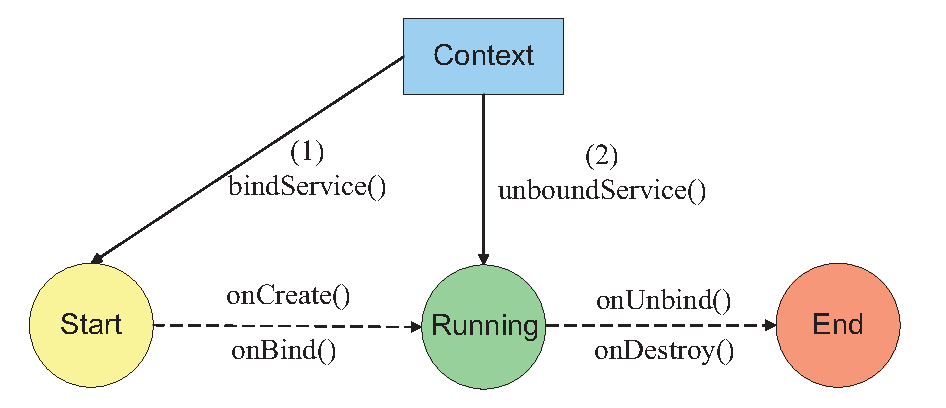
\includegraphics[scale=0.48]{bound.eps}}
  \caption{App service lifecycle: (a) started service, (b) bound service.}
\label{fig_lifecycle}
\end{figure}

\textbf{Started service}. The lifecycle of a started service is shown in Fig.~\ref{fig_lifecycle}a, which is explained as  follows. A started service is started via \hytt{Context.startService(Intent)} which triggers the system to retrieve the service or to create it via the \hytt{onCreate()} method of the service if the service has not been created yet, and then to invoke the \hytt{onStartCommand(Intent, int, int)} method of the service. The service keeps running until \hytt{Context.stopService()} or the \hytt{stopSelf()} method of the service is invoked. It is worth mentioning that if the service is not stopped, multiple invocations to \hytt{Context.startService()} result in multiple corresponding invocations to \hytt{onStartCommand()}, but do not create more service instances, that is, the service (instance) is shared by different callers. Once \hytt{Context.stopService()} or \hytt{stopSelf()} is invoked, the service is stopped and destroyed by the system via calling the \hytt{onDestroy()} method of the service, no matter how many times it was started.
However, if the \hytt{stopSelf(int)} method of the service is used, the service
will not be stopped until all started intents are processed.
Note that the started service and the components which start it are
loosely-coupled, i.e., the service can still keep running after the components
are destroyed.

\textbf{Bound service}. The lifecycle of a bound service is shown in
Fig.~\ref{fig_lifecycle}b. As started services cannot interact with the
components which start them, bound services are proposed, which can send data
to the launching components (clients). A client component can invoke
\hytt{Context.bindService()} to obtain a connection to a service. Similarly,
this creates the service by calling \hytt{onCreate()} without
\hytt{onStartCommand()} if it has not been created yet. A client component
receives the \hytt{IBinder} object (a client-server interface) which is returned
by the \hytt{onBind(Intent)} method of the service, allowing the two to
communicate. Although multiple client components can bind to the service, the
system invokes \hytt{onBind()} only once. The binding is terminated either
through the \hytt{Context.unbindService()} method (the system invokes
\hytt{onUnbind()}), or the client component's lifecycle ends. Thus, a bound
service is destroyed when no client components bind to it.

\textbf{Hybrid service}. A service can be both started and have connections
bound to it. This kind of services are referred to hybrid services.
A hybrid service can be started first and then bound, or vice versa. The
components that start and bind a hybrid service can be different.

\begin{table}
\centering
\caption{The Correlation Between Service Types and Service Usage Inefficiency Anti-patterns}
\small
\begin{tabular}{|c|c|c|c|c|}\hline
\multicolumn{2}{|c|}{\backslashbox{Anti-pattern}{Service type}}&Started &Bound&Hybrid
\\\hline
\multicolumn{2}{|c|}{Premature create} &   & $\surd$  &$\surd$
\\\hline
\multicolumn{2}{|c|}{Late destroy} & $\surd$& $\surd$&$\surd$
\\\hline
\multicolumn{2}{|c|}{Premature destroy} & $\surd$ & &$\surd$
\\\hline
\multicolumn{2}{|c|}{Service leak}& $\surd$& $\surd$& $\surd$
\\\hline
\end{tabular}
\label{tab_correlation}
\end{table}

\section{Service Usage Anti-Patterns}\label{antipatterns}
Based on the service lifecycle and our manual analysis of
real-world apps, we first present four anti-patterns that can lead to service usage
inefficiencies. It is worth mentioning that these four kinds of service usage
inefficiencies may occur to both local services (implemented by the app itself)
and remote services (implemented by other apps). We do not claim completeness of the four anti-patterns (there may exist other service usage inefficiencies, though we have not found any in our empirical study).
Table~\ref{tab_correlation} summarizes the four anti-patterns with respect to
different types of services.

\vspace{1ex}
\begin{pattern} [\textbf{Premature Create}] A service is created too early
before it is really used, and thus the service is in an idle state beginning
from its creation to its real use.
\label{p_prematurecreate}
\end{pattern}

Once a started service is started through \hytt{startService()}), \hytt{onCreate()} and \hytt{onStartCommand()} are invoked successively. Therefore, the use of started services is free of premature create bugs. The bugs of premature create can exist in the use of bound services: if a component binds a service but not immediately use the service (i.e., calls the methods of the service), then the service is created too early. For example, Figure~\ref{ex_precreate}a shows a premature create bug in the  \textit{Clean Master} app, where \hytt{NotificationManagerService} is bound too early before it is really used via \hytt{dZm.aqC()}, because there are other operations between these two operations.

The bugs of premature create occurring to the use of bound services may also occur to the use of hybrid services. Besides, hybrid services could be created even earlier: If the \hytt{onStartCommand()} method of the hybrid service is not overwritten, when the service is created by a \hytt{startService()} statement, the service will be in an idle state until it is used as a bound service. The code snippet in Fig.~\ref{ex_precreate}b reports such a premature create bug in the \textit{WhatsApp Messenger} app: The \hytt{onStartCommand()} method of the \hytt{GoogleDriveService} is not overwritten, and the \hytt{startService()} method is called but not directly followed by the \hytt{bindService()} method.

\begin{figure}
  \centering
 \subfigure[]{
    \lstinputlisting[language={Java}]{CleanMaster_PCB.java}}
  \subfigure[]{
    \lstinputlisting[language={Java}]{WhatsAppMessenger_PCB.java}}
  \caption{Real-world premature create bugs: (a) A premature create bug in \textit{Clean Master} (version 5.17.4), (b) A premature create bug in \textit{WhatsApp Messenger} (version 2.17.231).}
\label{ex_precreate}
\end{figure}

%A service in an idle state occupies unnecessary resources (e.g., memory) and consumes unnecessary energy, which reduces the performance of the app.

%Premature create can be formally described using the following LTL (\textit{linear temporal logic}) formula: $\square\neg overwritten(\hytt{onStartCommand()})$ $\wedge$ $\square$ ($\hytt{startService()}$ $\rightarrow$ $\bigcirc\neg \hytt{bindService()}$ $\wedge$ ($\neg \hytt{stopService()}$ \textsf{U} $\hytt{bindService()}$)).



\vspace{1ex}
\begin{pattern} [\textbf{Late Destroy}] A service is destroyed too late after its use, and thus the service is in an idle state beginning from the end of its final use to the moment it is destroyed.
\label{p_latedestroy}
\end{pattern}


Let us explain why the bugs of late destroy may exist. App services can be stopped (unbound) by end users via user-input events. Nevertheless, it only makes sense when end users want to stop (unbind) the services in advance. If end users want the services to complete the respective long-running tasks, they usually do not know the best moment to stop (unbind) the services. Besides, many services are non-interactive, i.e., they do not need user interaction at all~\cite{ZhangLLC17}. Therefore, the right time to stop (unbind) a service should be determined by the app itself.
More specifically,
\begin{enumerate}
\item The right time to stop a started service is to call \hytt{stopSelf()} or \hytt{stopSelf(int)} at the end of its \hytt{onStartCommand()} method, because the end represents that the service's task is finished. Otherwise, the service is  destroyed too late (stopped elsewhere), or not destroyed at all (cf. Anti-pattern~\ref{p_serviceleak}).
\item The right time to unbind a bound service is  at the moment when the communication between the client component  and the service is completed (i.e., the client component will not call the methods of the service any longer).
\item The right time to stop and to unbind a hybrid service is the same as that to stop a started service and to unbind a bound service, respectively.
\end{enumerate}

Figure~\ref{ex_lateDestroy} reports two late destroy bugs in real-world apps. The code snippet in Fig.~\ref{ex_lateDestroy}a reports a late destroy bug in the \textit{Twitter} app, where the \hytt{a()} method starts a service \hytt{OverlayService}. Despite the fact that the \hytt{stopService()} method is called in the \hytt{b()} method, the time to stop the \hytt{OverlayService} is too late. To address this problem, the \hytt{stopSelf()} method should be invoked in the \hytt{onStartCommand()} method of \hytt{OverlayService}. The code snippet in Fig.~\ref{ex_lateDestroy}b shows a late destroy bug in the \textit{YouTube} app, where the class \hytt{ahx} binds a service from a third
party. The \hytt{bindService()} method is called in the \hytt{d()} method of
\hytt{ahx}, but the corresponding \hytt{unbindService()} method is not called
immediately after the last invocation of the method (i.e.,~\hytt{post()}) of the
service in \hytt{f()}. The service remains idle until the \hytt{e()} method of
\hytt{ahx} is called.

\begin{figure}
  \centering
  \subfigure[]{
    \lstinputlisting[language={Java}]{Twitter_LDB.java}}
  \subfigure[]{
    \lstinputlisting[language={Java}]{YouTube_LDB.java}}
  \caption{Real-world late destroy bugs: (a) A late destroy bug in \textit{Twitter} (version 7.0.0), (b) A late destroy bug in \textit{YouTube} (version 12.23.60).}
\label{ex_lateDestroy}
\end{figure}


\vspace{1ex}
\begin{pattern} [\textbf{Premature Destroy}] Suppose that a service is used simultaneously by several components. The service is destroyed too early if one component destroys it before another component begins to use it, and thus it has to be recreated.
\label{p_prematuredestroy}
\end{pattern}

Anti-pattern~\ref{p_prematuredestroy} can occur to started services and hybrid
services. If there are several components that can start a service
simultaneously, \hytt{stopSelf(int startID)} should be called in
\hytt{onStartCommand()}. This guarantees that the service is not destroyed if the argument \hytt{startID} is not the same as that generated by the last start of the service. However, if \hytt{stopSelf()} is used instead, the created service may be destroyed too early before other components' use. Consequently, the service should be created again to respond to other components.
The premature destroy bugs lead to many unnecessary destroy and recreation of
the same service, reducing the performance of the apps significantly.

\begin{figure}
  \centering
    \lstinputlisting[language={Java}]{WhatsAppMessenger_PDB.java}
  \caption{A real-world premature destroy bug in \textit{WhatsApp Messenger} (version 2.17.231).}
\label{ex_predestroy}
\end{figure}


%To determine whether an app involves the bugs of premature destroy, the crux is to check whether there are two or more components that share the same services.

Bound services are destroyed once they become unbounded.
If a service becomes unbounded, it indicates that all client components which bound it have finished using it.
In other words, at that moment there is no other client component which is
using it or ready to use it. Therefore, bound services are free of the premature
destroy bugs by nature.

Figure~\ref{ex_predestroy} reports a premature destroy bug in the \textit{WhatsApp Messenger} app: The \hytt{startService()} method of  \hytt{MessageService} is called three times, but  \hytt{stopSelf()} (instead of \hytt{stopSelf(int)}) is used in the \hytt{onStartCommand()} method of \hytt{MessageService}.

%Similar to started services, the use of hybrid services may also involves the bugs of premature destroy, when \hytt{stopSelf()} instead of \hytt{stopSelf(int)} is used in \hytt{onStartCommand()} and no component .
%
\vspace{1ex}
\begin{pattern} [\textbf{Service Leak}] A service is never destroyed after its use, even when the apps which use the service terminate.
\label{p_serviceleak}
\end{pattern}



Anti-pattern~\ref{p_serviceleak} refers to the bugs that the services are never
destroyed except for the situation that they are stopped (unbound) by end users.
However, as aforementioned, the programmers should not rely on end users to stop
(unbind) the app services but, instead, the services should be stopped
(unbound) by the app itself. If a service is started (bound) but is not stopped
(unbound), the service is leaked. As started services execute in an
isolated process, a leaked service can keep running even after the app process
has terminated, which may cause severe performance issues in the long run.
%The service leak bugs are more severe than the late destroy bugs.

Despite the fact that the leaked services and the services destroyed too late
(but not destroyed yet) can be automatically killed by the system when the
system resource (e.g., memory) becomes low, the started services which were
killed can be rebooted later, if the return value of their
\hytt{onStartCommand()} method is ``\hytt{START\_STICKY}'' or
``\hytt{START\_REDELIVER\_INTENT}''. In addition, since the leaked services can
occupy much memory, normal services may be unexpectedly killed by the system.
Note that Android 8.0 has taken actions on limiting background services: when
the app is not in the foreground, the app's background services are stopped by
the system. This may alleviate the impact of late destroy and service leak, but
cannot avoid them. Moreover, this cannot prevent premature create and premature
destroy.


Fig.~\ref{ex_leak} reports two service leak bugs in real-world apps. The code snippet in Fig.~\ref{ex_leak}a shows a service leak bug in the \textit{Messenger} app: The \hytt{startService()} method that starts the service \hytt{MpService} is called in the \hytt{a()} method of the class \hytt{MpActivity}, but, the corresponding \hytt{stopService()} method is called only when the \hytt{b()} method returns ``true''. The code snippet in Fig.~\ref{ex_leak}b shows a service leak bug in the  \textit{Google Play Music} app: the service \hytt{ArtDownloadService} is bound through \hytt{ArtMonitorImpl} but is never unbound.

\begin{figure}
  \centering
 \subfigure[]{
    \lstinputlisting[language={Java}]{Messenger_SLB.java}}
  \subfigure[]{
    \lstinputlisting[language={Java}]{GooglePlayMusic_SLB.java}}
  \caption{Real-world service leak bugs: (a) A service leak bug in \textit{Messenger} (version 123.0.0.11.70), (b) A service leak bug in \textit{Google Play Music} (version 7.8.4818-1.R.4063206).}
\label{ex_leak}
\end{figure}


\section{Detecting Service Usage Bugs}\label{approach}
Based on the four anti-patterns, we present a
static analysis to detect service usage inefficiency bugs in Android apps.
To scale to large real-world apps, we use a context-insensitive,
but path-sensitive inter-procedural control flow analysis.

Since some services declared in the AndroidManifest file may not
be implemented or used in the app code, we only consider the services
that are actually implemented or used. Note that the service types
cannot be determined directly from the AndroidManifest file or the service
definition (i.e., the class that defines the service). We have to determine the
service type according to all uses of the service from the app code. If a
service is only initiated through \hytt{startService()} (\hytt{bindService()}),
it is a started (bound) service; otherwise, it is a hybrid service.
According to the service types, we then determine whether there
are use cases of the services that may lead to corresponding service usage
inefficiencies. Our analysis covers all usage of each service.

Fig.~\ref{fig_framework} illustrates the framework of our approach, which
includes three main modules:
\begin{enumerate}
\item \textit{Service Identifier}: For each statement of service use (e.g., \hytt{startService(intent)},  \hytt{bindService(intent)}, \hytt{stopService(intent)}), this module identifies the corresponding service $s$ according to the argument $intent$. If $intent$ is explicit, $s$ is obtained from $intent$'s API invocations, e.g., \hytt{intent.setClass(context, cls)}, \hytt{intent.setClassName(context, cls)}, or \hytt{intent.setComponent(comp)}~\cite{Androidintentfilter}. If $intent$ is implicit, $s$ is obtained from the matched $<$intent-filter/$>$ defined in the AndroidManifest XML file~\cite{Androidintentfilter}.
\item \textit{Component Identifier}: For each statement of service use, say, \hytt{startService(intent)}, this module identifies the component $c$ that uses the service by back tracking the call graph starting from the statement (node) \hytt{startService(intent)}. The call graph is generated by \textsf{Soot}~\cite{sootpaper}.
\item \textit{Bug Detector}: The app control flow graph (CFG) can be generated by \textsf{Soot}. For each service use, since the component $c$ and the service $s$ are known, according to the CFG, \textit{Bug Detector} determine whether or not this service use may lead to service usage inefficiency bugs. Since this is the crucial module of \textsf{ServDroid}, we next present our analysis for detecting each of the four kinds of bugs in more detail.
\end{enumerate}


 \begin{figure}
 \centering
  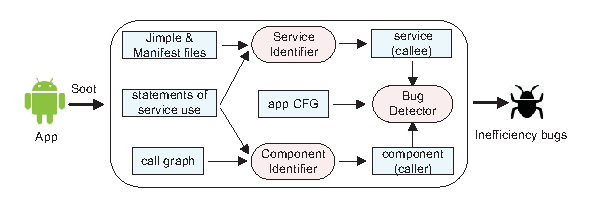
\includegraphics[scale=0.95]{framework.eps}
 \caption{Approach framework of \textsf{ServDroid}.}
\label{fig_framework}
\end{figure}

\subsection{Detecting Premature Create Bugs}
As mentioned in Section~\ref{antipatterns}, there are two kinds of premature create bugs. The first kind can occur to the usage of bound services and hybrid services, whereas the second kind can only occur to the usage of hybrid services.

We first discuss how to detect the first kind of premature create bugs. We search in the CFG of the app for all the \hytt{bindService()} statements. For each \hytt{bindService()} statement $stm_b$ in the CFG, we first determine the client component $c$ and the bound service $s$ such that $c$ binds $s$ through $stm_b$. Then, from the CFG, we find a successor $stm_u$ of $stm_b$ such that $stm_u$ is the first statement that $c$ invokes a method of $s$. If there is no statements between $stm_b$ and $stm_u$ that are relevant to $c$ (invoked by $c$), $c$'s use of $s$ is free of premature create bugs. Otherwise, there is a premature create bug, i.e., $c$ binds $s$ too early.

Let us return to the example in Figure~\ref{ex_precreate}a. Since \hytt{dZm.aqC()} is the first statement that $c$ uses $s$, and there are other operations invoked by $c$ (e.g., \hytt{oj()}, \hytt{arF()}) between \hytt{context.bindService()} and \hytt{dZm.aqC()} in the CFG, a premature create bug is found.

We then discuss how to detect the second kind of premature create bugs.  We first check whether the
\hytt{onStartCommand()} method of the service $s$ is overwritten. If it is
overwritten, the service usage does not involve premature create bugs.
Otherwise, we check whether there is a path in the CFG of the app such that
the following two conditions are satisfied (if both conditions are satisfied,
the service $s$ involves premature create bugs):
\begin{enumerate}
\item No component binds to service $s$ when the \hytt{startService()} statement is executed.
\item There is a \hytt{bindService()} statement which follows but not
immediately follows the \hytt{startService()} statement (i.e., \hytt{bindService()} is a successor but not a direct successor of \hytt{startService()} in the CFG) and there is no corresponding \hytt{stopService()} between \hytt{startService()} and \hytt{bindService()}.
\end{enumerate}

To check the first condition, we first obtain the dominators (cf.
Definition~\ref{def_dom}) of the \hytt{startService()} statement $stm_s$. If the
list of dominators does not include a \hytt{bindService()} statement $stm_b$ that binds the same service $s$,
the first condition is satisfied. Otherwise, we further check whether the
corresponding \hytt{unbindService()} statement follows $stm_b$ in the CFG, or
the component that binds $s$ is destroyed before $stm_s$. If either is met, the first condition is satisfied. For the second condition, we check whether there is a  \hytt{bindService()} statement $stm_{b_1}$ that is the transitive successor of $stm_s$. If yes, we further check each path from $stm_s$ to $stm_{b_1}$. If there is no \hytt{bindService()} statement that is the direct successor of $stm_s$, and there is no  \hytt{stopService()} statement that stops $s$, the second condition is satisfied.


\begin{definition}[\textbf{Dominator}]
  In a CFG, a node (statement) $s_j$ is dominated by another node
  $s_i$ if every path from the entry of the CFG to $s_j$
  contains $s_i$. $s_i$ is called a dominator of $s_j$.
\label{def_dom}
\end{definition}

Let us return to the example in Figure~\ref{ex_precreate}b. Since \hytt{onStartCommand()} is not overwritten, and the component has other operations (e.g., \hytt{q()}) between \hytt{startService()} and \hytt{bindService()} in the CFG, a premature create bug is found.


\subsection{Detecting Late Destroy Bugs}

For a started service, its use involves a late destroy bug if
\hytt{stopSelf()} or \hytt{stopSelf(int)} is not called in the
\hytt{onStartCommand()} method of the service. Hence, the detection is straightforward.

We elaborate on how to detect late destroy bugs occurring to the use of bound services. We search in the CFG of the app for all the \hytt{unbindService()} statements. For each \hytt{unbindService()} statement $stm_{un}$ in the CFG, we first determine the client component $c$ and the bound service $s$ such that $c$ unbinds $s$ through $stm_{un}$. Then, from the CFG, we find a precursor $stm_u$ of $stm_{un}$ such that $stm_u$ is the last statement that $c$ invokes a method of $s$. If there is no statements between $stm_u$ and $stm_{un}$ that are relevant to $c$ (invoked by $c$), $c$'s use of $s$ is free of late destroy bugs. Otherwise, there is a late destroy bug, i.e., $c$ unbinds $s$ too late.

For the example in Figure~\ref{ex_lateDestroy}b, the invocation of \hytt{f()} corresponds to the last use of the service $s$, and the invocation of \hytt{e()} is to unbind $s$. Since other operations (e.g., \hytt{c()}) between these two invocations are found from the CFG, a late destroy bug is detected.

For hybrid services, we combine the above two methods (applying to started services and bound services, respectively) to determine whether their usage may involve late destroy bugs.

\subsection{Detecting Premature Destroy Bugs}
The use of a started or a hybrid service may involve premature destroy bugs, if
the service is shared by two or more components (callers), and \hytt{stopSelf()}
instead of \hytt{stopSelf(int)} is called in the \hytt{onStartCommand()} method
of the service. Therefore, the method of detecting premature destroy bugs is straightforward.



\subsection{Detecting Service Leak Bugs}
Normally, to bind a service, each bind statement should have a corresponding
unbind statement such that the callers (client components) of the two statements
are the same. However, to start a service, multiple start statements may
correspond to the same (only one) stop statement. If a start (bind) statement is not always
followed by a stop (unbind) statement, the service may leak. As aforesaid, no
matter whether end users can destroy a service or not, the app itself should
have the mechanism to destroy the created service.  With that in mind, we have
the following steps to determine whether a service may leak:

\begin{enumerate}
\item We first find all statements that start (bind) the service, i.e.,
\hytt{startService()} (\hytt{bindService()}). All such statements are summarized
in a set $S_1$.
\item We then find all statements that stop (unbind) the same service, i.e., \hytt{stopService()} (\hytt{unbindService()}). All the  statements are summarized in a set $S_2$.
\item We next remove from $S_2$ the statements that are triggered by end users,
i.e., the statements that are triggered by the event handlers (callbacks) of the UI events (e.g., user click).
\item For each start (bind) statement in $S_1$, we check whether the
corresponding stop (unbind) statement exists in $S_2$. If not, the service leaks. If yes, we further determine whether
the stop (unbind) statement can be always reached from the corresponding start
(bind) statement. If not, the service also leaks.
\end{enumerate}

In the last step above, it is challenging to precisely determine whether a stop
(unbind) statement $stm_2$ can always be reached from the corresponding start (bind)
statement $stm_1$. To balance precision and efficiency, our
method is based on \textit{post-dominator} (cf. Definition~\ref{def_postdom}):
if $stm_2$ is a post-dominator of $stm_1$ in the (context-insensitive) CFG of the app, then the service does not leak. Otherwise, it may leak.

\begin{definition}[\textbf{Post-dominator}]
  In a CFG, a node (statement) $s_i$ is post-dominated by another
  node $s_j$ if each directed path from $s_i$ to the exit (return
  statement) of the CFG contains $s_j$. $s_j$ is called a
  post-dominator of $s_i$.
\label{def_postdom}
\end{definition}

Let us return to the example in Figure~\ref{ex_leak}a. In the CFG of \textsf{Messenger}, since the \hytt{startService()} method is not post-dominated by the \hytt{stopService()} method, a service leak bug is found.

\vspace{1ex}
Our detection for each anti-pattern is complete. For each service, \textsf{ServDroid} examines its uses along all potential paths, and all uses of all services are examined statically. To improve the analysis accuracy for real-world apps, we also take the following
two steps in the analysis:
\begin{enumerate}
\item Since a service is used by another component through the \textit{intent}
object (e.g., via \hytt{Intent intent = new Intent (Context, Class$<$?$>$
Service)}), the definition (i.e., class) of the service needs to be found
according to the \textit{intent}. Besides \textit{Service.class}, developers
also often use the reflection mechanism \hytt{Class.forName(Service)} to get the
service class object. Thus, we consider both ways to find
the service class.
\item Since the \textit{intent} object that is used to initiate a service (e.g.,
via \hytt{startService(Intent intent)}) can be created in a nested method whose
nesting depth may be large (e.g., bigger than 10), we set a
large threshold ($depth$ = 50) for the search loop to make sure that the
innermost method can be found while the efficiency is guaranteed.
\end{enumerate}

\section{Empirical Evaluation}\label{evaluation}
In this section, we study service usage inefficiencies in real-world popular
Android apps, aiming to answer the following research questions:

\begin{itemize}
\item {\bf RQ1} - {\it Performance of \textsf{ServDroid}}: What are the
precision, recall, and time overhead of \textsf{ServDroid}?
\item {\bf RQ2} - {\it Energy savings}: How much energy can be saved if these
services usage inefficiency bugs are fixed?
\item {\bf RQ3} - {\it Service usage frequency}: Are background services widely
used in Android apps? Which type of services are used most frequently?
\item {\bf RQ4} - {\it Pervasiveness of inefficiency bugs}: Are service usage inefficiency bugs common in practice?
\item {\bf RQ5} - {\it Distribution of inefficiency bugs}: How are the four kinds of service usage inefficiency bugs distributed in the three types of services?
\item {\bf RQ6} - {\it Dominating inefficiency bugs}: Among the four kinds of service usage inefficiency bugs, which kind is the most prevalent?
\item {\bf RQ7} - {\it Most vulnerable service type}: Among the three types of services, the usage of which type is more prone to inefficiency bugs?
\end{itemize}

All apps are analyzed with \textsf{ServDroid} on a computer with an Intel Core i7 3.6GHz CPU and 16 GB of memory, running Windows 8, JDK 1.7, and Android 7.0, 7.1.1, and 8.0.

%In the evaluation, we use both a manual inspection and a software tool (i.e., our prototype \textsf{ServDroid}) to analyze the service usage inefficiency bugs in these apps.
\subsection{Experiments on 45 Apps}

\subsubsection{Experimental Setup}
We first conduct an experimental evaluation on the top 45 most
downloaded free Android apps according to Wikipedia. The first 25 apps have
over one billion downloads and the rest 20 apps all have over 500 million
downloads. The first two columns of Table~\ref{tab_resultsum} respectively
report the names of these 45 apps and their versions we use. It is worth
mentioning that all the app versions were the latest in early January, 2018.

\textbf{Oracle}. We conducted an empirical study on these 45 apps by manual
inspection. Using the reverse engineering tools (\textsf{dex2jar}\footnote{https://sourceforge.net/projects/dex2jar} and \textsf{jd-gui}\footnote{http://jd.benow.ca}), each APK file was transformed into Java code, and three graduate students who mastered the four anti-patterns manually and independently searched the bugs in the source code. The inconsistencies among them were solved through iterative checking and coordination. The inspection took them about two weeks. We use the code inspection
results as the oracle (ground truth) to evaluate the effectiveness of our approach.

\textbf{Implementation}. We implemented our approach in an open-source prototype
tool {\sf ServDroid} based on {\sf Soot}~\cite{sootpaper}. The input of {\sf
ServDroid} is an app (APK file), and its output is the detected service usage
inefficiency bugs in the app. {\sf ServDroid} also returns the calling context to
help debug these inefficiencies. We also use {\sf ServDroid} to
detect the service usage inefficiency bugs in these 45 apps, and compare the
detected results with those of the manual inspection.

\begin{table*}
\centering
%\footnotesize
\small
\caption{Total Number of Services and Service Usage Inefficiency Bugs}
\begin{tabular}{|l|c|cccc|ccccc|}\hline
{\bf App name}&\multicolumn{1}{|c|}{\textbf{Version}}&\multicolumn{4}{|c|}{\textbf{\# Services}} &\multicolumn{5}{|c|}{\textbf{\# Service usage inefficiency bugs}}\\
&{\bf }&{\bf Started}&{\bf Bound}&{\bf Hybrid} &{\bf Total} & {\bf PCBs}&{\bf LDBs}&{\bf PDBs} &{\bf SLBs}&{\bf Total}\\
\hline
\hline
{\it Google Play services} & 11.0.55 (436-156917137) & {\bf 130} & {\bf 17} & 6 & {\bf 153} & {\bf 6 }& 4 & 0 & {\bf 95} & {\bf 105}\\
{\it Gmail} & 7.6.4.158567011.release & 18 & 2 & 4 & 24 & 1 & 1 & 0 & 5 & 7\\
{\it Maps} & 9.54.1 & 12 & 9 & 4 & 25 & 2 & 1 & 1 & 9 & 13\\
{\it YouTube} & 12.23.60 & 10 & 2 & 3 & 15 & 2 & 2 & 0 & 3 & 7\\
{\it Facebook} & 10.2.0 & 22 & 8 & 4 & 34 & 0 & 4 & 0 & 5 & 9\\
{\it Google} & 7.3.25.21.arm & 21 & 10 & 6 & 37 & 5 & 3 & 0 & 1 & 9\\
{\it Google+} & 9.14.0.158314320 & 23 & 1 & 4 & 28 & 0 & 1 & 0 & 7 & 8\\
{\it GoogleText-to-Speech} & 3.11.12 & 4 & 1 & 0 & 5 & 0 & 0 & 0 & 2 & 2\\
{\it WhatsApp Messenger} & 2.17.231 & 9 & 5 & 5 & 19 &  5 & 2 & {\bf 2} & 10 & 19\\
{\it Google Play Books} & 3.13.17 & 8 & 2 & 1 & 11 & 0 & 0 & 0 & 1 & 1\\
{\it Messenger} & 123.0.0.11.70 & 40 & 1 & 0 & 41 & 0 & 1 & 0 & 9 & 10\\
{\it Hangouts} & 20.0.156935076 & 11 & 9 & 2 & 22 & 0 & 1 & 1 & 4 & 6\\
{\it Google Chrome} & 58.0.3029.83 & 16 & 9 & 2 & 27 & 0 & 0 & 0 & 0 & 0\\
{\it Google Play Games} & 3.9.08(3448271-036) & 4 & 0 & 0 & 4 & 0 & 0 & 0 & 3 & 3\\
{\it Google TalkBack} & 5.2.0 & 2 & 1 & 0 & 3 & 0 & 0 & 0 & 1 & 1\\
{\it Google Play Music} & 7.8.4818-1.R.4063206 & 15 & 3 & 4 & 22 & 1 & 3 & 1 & 10 & 15\\
{\it Google Play Newsstand} & 4.5.0 & 8 & 1 & 1 & 10 & 0 & 1 & 1 & 3 & 5\\
{\it Google Play Movies \&  TV} & 3.26.5 & 6 & 4 & 2 & 12 & 0 & 0 & 0 & 4 & 4\\
{\it Google Drive} & 2.7.153.14.34 & 6 & 6 & 3 & 15 & 1 & 2 & 0 & 3 & 6\\
{\it Samsung Push Service} & 1.8.02 & 11 & 0 & 0 & 11 & 0 & 3 & 0 & 1 & 4\\
{\it Instagram} & 10.26.0 & 14 & 4 & 2 & 20 & 3 & 1 & 0 & 7 & 11\\
{\it Android System WebView} & 58.0.3029.83 & 8 & 2 & 1 & 11 & 0 & 0 & 0 & 0 & 0\\
{\it Google Photos} & 2.16.0.157775819 & 17 & 8 & 6 & 31 & 3 & 2 & 1 & 4 & 10\\
{\it Google Street View} & 2.0.0.157538376 & 6 & 5 & 2 & 13 & 0 & 4 & 0 & 8 & 12\\
{\it Skype} & 8.0.0.44736 & 10 & 1 & 0 & 11 & 0 & 0 & 0 & 0 & 0\\
{\it Clean Master} & 5.17.4 & 20 & 16 & 3 & 39 & 3 & {\bf 10} & 2 & 26 & 41\\
{\it Subway Surfers} & 1.72.1 & 2 & 1 & 0 & 3 & 0 & 0 & 0 & 1 & 1\\
{\it Dropbox} & 50.2.2 & 8 & 3 & 1 & 12 & 2 & 1 & 1 & 4 & 8\\
{\it Candy Crush Saga} & 1.101.0.2 & 2 & 1 & 1 & 4 & 0 & 1 & 0 & 0 & 1\\
{\it Viber Messenger} & 8.0.0.3 & 8 & 6 & 3 & 17 & 4 & 3 & 0 & 5 & 12\\
{\it Twitter} & 7.0.0 & 9 & 2 & 2 & 13 & 0 & 1 & 0 & 3 & 4\\
{\it LINE} & 7.5.2 & 11 & 5 & 3 & 19 & 3 & 1 & 1 & 12 & 17\\
{\it HP Print Service Plugin} & 3.4-2.3.0 & 4 & 3 & 2 & 9 & 1 & 1 & 0 & 5 & 7\\
{\it Flipboard} & 4.0.13 & 4 & 3 & 3 & 10 & 0 & 1 & 0 & 3 & 4\\
{\it Samsung Print Service Plugin} & 3.02.170302 & 7 & 3 & 0 & 10 & 1 & 2 & 0 & 6 & 9\\
{\it Super-Bright LED Flashlight} & 1.1.7 & 5 & 0 & 4 & 9 & 0 & 2 & 0 & 7 & 9\\
{\it Gboard} & 6.3.28.159021150 & 6 & 4 & 2 & 12 & 1 & 0 & 0 & 2 & 3\\
{\it Cloud Print} & 1.36b & 8 & 1 & 1 & 10 & 0 & 2 & 0 & 1 & 3\\
{\it Snapchat} & 10.10.5.0 & 6 & 3 & 0 & 9 & 1 & 5 & 1 & 2 & 9\\
{\it Pou} & 1.4.73 & 4 & 0 & 0 & 4 & 0 & 2 & 0 & 2 & 4\\
{\it Google Translate} & 5.9.0.RC07.155715800 & 6 & 0 & 1 & 7 & 1 & 4 & 0 & 3 & 8\\
{\it My Talking Tom} & 4.2.1.50 & 17 & 6 & 2 & 25 & 0 & 3 & 2 & 13 & 18\\
{\it Security Master} & 3.4.1 & 7 & 3 & 4 & 14 & 3 & 2 & 2 & 7 & 14\\
{\it Facebook Lite} & 20.0.15 & 20 & 9 & 4 & 33 & 1 & 9 & 2 & 7 & 19 \\
{\it imo messenger} & 11.3.2 & 16 & 6 & {\bf 7} & 29 & 5 & 4 & 1 & 14 & 24\\
\hline
{\bf Sum} & - &  601  & 186  &  105  &  892 & 55 & 90 & 19 & 318 & 482\\
\hline
%{\bf Average} & 0.4 & 2.0 & 0.4 & 6.8 & 9.6 & $\_$ & $\_$ \\
{\bf Average} & - & 13.4  &   4.1  &   2.3  &   19.8 & 1.2 & 2.0 & 0.4 & 7.1 & 10.7\\
\hline
\end{tabular}
\label{tab_resultsum}
\end{table*}


\subsubsection{Experimental Results}

The third column of Table~\ref{tab_resultsum} summarizes the numbers
of different types of services used in the 45 Android apps. The last column of Table~\ref{tab_resultsum}
summarizes the numbers of premature create bugs (PCBs), late destroy bugs
(LDBs), premature destroy bugs (PDBs), service leak bugs (SLBs), and all service usage
inefficiency bugs detected by \textsf{ServDroid} in the 45 apps.
Taking the manual inspection results as ground truth, the
accuracy of \textsf{ServDroid} is reported as follows.

\medskip
%\setlength{\fboxrule}{0.7 pt}
%\setlength{\fboxsep}{0.2 cm}
{\setlength{\parindent}{0 em}
\fbox{\begin{minipage}{3.23 in}
{\bf Answer to RQ1:}
The overall precision and recall of the results returned by \textsf{ServDroid}
are both 100\%. The total runtime overhead of {\sf ServDroid} on analyzing the
45 apps is 4,325 seconds, with about 96 seconds on average to analyze one app.\\
{\bf Implication:}
The lightweight analysis of \textsf{ServDroid} for detecting such particular
anti-patterns has a high accuracy, and is scalable.
\end{minipage}}
}\\
\medskip

The high accuracy of \textsf{ServDroid} indicates that its ability to detect
service usage inefficiency bugs is not undermined by the context-insensitive
analysis.


To investigate the energy impact of the inefficiency bugs, we first use
\textsf{Soot} to instrument the infected apps to fix the inefficiency bugs (the details are beyond the scope of this paper), and
repackage them. Then, we run the original and repackaged apps independently on a
phone (Google Nexus 6P, running Android 8.0) with the same setting (e.g., user operations) for 15 minutes\footnote{It is sufficient to see the difference of battery cost.}, and use the tool (also an app)
\textsf{Trepn Profiler} to measure the battery cost of them, respectively. Based on the static analysis result of \textsf{servDroid}, we make sure that the behavior of the app related to the service inefficiency bugs is exercised. The above measurement is repeated three times. The
average battery cost is summarized in Table~\ref{tab_energy}, including the data of 38 apps (the other seven
apps are not measured because they are either free of the inefficiency bugs or cannot run
independently).
Based on the results in Table~\ref{tab_energy}, we have the following finding:

\medskip
%\setlength{\fboxrule}{0.7 pt}
%\setlength{\fboxsep}{0.2 cm}
{\setlength{\parindent}{0 em}
\fbox{\begin{minipage}{3.23 in}
{\bf Answer to RQ2:}
The average energy consumptions (15 minutes) of an app before and after the service usage inefficiency bugs are fixed are 546.73 Joule and 459.59 Joule, respectively. That is, an app can save on average 87.14 Joule in 15 minutes if the bugs are fixed.\\
{\bf Implication:}
The energy consumption is reduced after the bugs are fixed, and thus the
inefficiency bugs have a significant impact on energy consumption.
\end{minipage}}
}\\
\medskip

\begin{table}
\centering
\small
\caption{Energy Consumption Before and After the Bugs Are Fixed}
\begin{tabular}{|l|cc|}\hline
{\bf App name}&\multicolumn{2}{|c|}{\textbf{Energy consumption}}\\
& {\bf Original (J)}&{\bf Repaired (J)}\\
\hline
\hline
{\it Google Play services}&574.68&373.42\\
{\it Gmail}&437.05&388.25\\
{\it Maps}&626.67&487.28\\
{\it YouTube}&803.31&687.05\\
{\it Facebook}&553.94&510.34\\
{\it Google}&498.40&426.82\\
{\it Google+}&438.59&422.57\\
{\it GoogleText-to-Speech}&395.90&353.91\\
{\it WhatsApp Messenger}&421.93&343.58\\
{\it Google Play Books}&474.77&435.57\\
{\it Messenger}&509.60&412.92\\
{\it Hangouts}&370.33&338.30\\
%{\it Google Chrome}&492.35&492.35\\
{\it Google Play Games}&549.86&475.03\\
{\it Google TalkBack}&458.57&429.97\\
{\it Google Play Music}&567.35&458.59\\
{\it Google Play Newsstand}&512.50&442.20\\
{\it Google Play Movies \& TV}&363.39&317.45\\
{\it Google Drive}&338.49&286.74\\
%{\it Samsung Push Service}&597.97&529.01\\
{\it Instagram}&496.44&452.05\\
%{\it Android System WebView}&573.29&493.72\\
{\it Google Photos}&484.75&435.66\\
{\it Google Street View}&424.91&369.53\\
%{\it Skype}&479.15&479.15\\
{\it Clean Master}&482.36&399.24\\
{\it Subway Surfers}&950.96&899.31\\
{\it Dropbox}&462.38&408.53\\
{\it Candy Crush Saga}&820.80&557.36\\
{\it Viber Messenger}&483.64&419.39\\
{\it Twitter}&588.59&537.88\\
{\it LINE}&572.07&497.71\\
%{\it HP Print Service Plugin}&471.62&420.18\\
{\it Flipboard}&486.41&438.67\\
%{\it Samsung Print Service Plugin}&508.62&459.3\\
{\it Super-Bright LED Flashlight}&454.12&385.26\\
{\it Gboard}&497.44&441.62\\
%{\it Cloud Print}&602.51&517.13\\
{\it Snapchat}&611.63&461.71\\
{\it Pou}&1,000.41&647.33\\
{\it Google Translate}&378.40&342.36\\
{\it My Talking Tom}&1,432.49&1,197.11\\
{\it Security Master}&437.09&368.08\\
{\it Facebook Lite}&362.16&297.52\\
{\it imo messenger}&492.46&325.50\\
\hline
%{\bf Sum}&25752.2&21674.15\\
{\bf Sum}&20,814.81&17,471.82\\
\hline
%{\bf Average}&572.27&481.64\\
{\bf Average}&547.76&459.78\\
\hline
\end{tabular}
\label{tab_energy}
\end{table}


\subsection{Empirical Study}

Since the precision and recall of \textsf{servDroid} are both 100\%, using \textsf{servDroid}, we conduct an empirical
study on 1,000 Android apps randomly selected from Google play (accessed in Dec 2018), to extensively study the service usage and the relevant inefficiency bugs in practice. From the 1,000 Android apps, we have the following findings.

%\begin{table*}
%\centering
%\footnotesize
%\caption{Services and Service Usage Efficiency Bugs of 1,000 Apps}
%\begin{tabular}{|c|c|cc|ccccc|}\hline
%{\bf \# Apps }&\multicolumn{1}{|c|}{\bf \# Apps using services}&\multicolumn{2}{|c|}{\textbf{Service type}} &\multicolumn{5}{|c|}{\textbf{\# Service usage inefficiency bugs}}\\
%&{\bf }&{\bf Type}&{\bf Number}& {\bf PCBs}&{\bf LDBs}&{\bf PDBs} &{\bf SLBs}&{\bf Total}\\\hline
%\hline
%       \multirow{3}{*}{1,000}& \multirow{3}{*}{939} &{\textbf{Started}} & 4,952& 0 & 491 & 137& 1,720 & 2,348\\
%
%                & & {\textbf{Bound}} & 2,468 & 400 & 620 & 0 & 392 & 1,412\\
%
%                & & {\textbf{Hybrid}} & 715 & 163 & 175 & 38 & 290 & 666\\
%\hline
%\end{tabular}
%\label{tab_1000}
%\end{table*}

\medskip
%\setlength{\fboxrule}{0.7 pt}
%\setlength{\fboxsep}{0.2 cm}
{\setlength{\parindent}{0 em}
\fbox{\begin{minipage}{3.23 in}
{\bf Answer to RQ3:}
Among the 1,000 apps, 939 use background services. The total numbers (proportions) of started, bound, and hybrid services in these apps are 4,952 (60.87\%), 2,468 (30.34\%), 715 (8.79\%), respectively. Each app uses about 8 services on average. \\
{\bf Implication:}
Services are widely used in Android apps, and started services are the most frequently used type of services.
\end{minipage}}
}\\
\medskip

%The reason why started services are the most frequently used type of services lies in that they require less user interaction that the other types of services, and are thus more suitable for time-consuming tasks running in the background.




\medskip
%\setlength{\fboxrule}{0.7 pt}
%\setlength{\fboxsep}{0.2 cm}
{\setlength{\parindent}{0 em}
\fbox{\begin{minipage}{3.23 in}
{\bf Answer to RQ4:}
Surprisingly, service usage inefficiency bugs are common in the 1,000 Android apps. 825 (82.5\%) of them are infected by at least one kind of efficiency bug; 608 (60.8\%) of them involve at least two kinds of inefficiency bugs; 304 (30.4\%) of them have no less than three kinds of inefficiency bugs; and 59 (5.9\%) of them are found to have all the four kinds of inefficiency bugs. Each app has 4.43 bugs on average.\\
{\bf Implication:}
Service usage inefficiency bugs are common in real-world popular Android apps.
\end{minipage}}
}\\
\medskip


\medskip
%\setlength{\fboxrule}{0.7 pt}
%\setlength{\fboxsep}{0.2 cm}
{\setlength{\parindent}{0 em}
\fbox{\begin{minipage}{3.23 in}
{\bf Answer to RQ5:}
The numbers (proportions) of premature create bugs occurring on the started services, bound services, and hybrid services are 0 (0\%), 400 (71.05\%), and 163 (28.95\%), respectively. The numbers (proportions) of late destroy bugs occurring on the started services, bound services, and hybrid services are 491 (38.18\%), 620 (48.21\%), and 175 (13.61\%), respectively. The numbers (proportions) of premature destroy bugs occurring on the started services, bound services, and hybrid services are 137 (78.29\%), 0 (0\%), and 38 (21.71\%), respectively. The numbers (proportions) of service leak bugs occurring on the started services, bound services, and hybrid services are 1,720 (71.61\%), 392 (16.32\%), and 290 (12.07\%), respectively.\\
{\bf Implication:}
This confirms the analysis results in Table~\ref{tab_correlation} that the
premature create bugs do not occur on the usage of started services; premature destroy
bugs do not occur on the usage of bound services; late destroy bugs and service
leak bugs can happen to all the three types of services.
\end{minipage}}
}\\
\medskip

\iffalse
\medskip
%\setlength{\fboxrule}{0.7 pt}
%\setlength{\fboxsep}{0.2 cm}
{\setlength{\parindent}{0 em}
\fbox{\begin{minipage}{3.23 in}
{\bf Answer to RQ6:}
Among the 1,0000 apps, 137 have premature create bugs, 981 are infected by late destroy bugs, 160 are found to have premature destroy bugs, and 2,089 involve service leak bugs; the proportion of the four kinds of bugs are 4.07\%, 29.14\%, 4.75\%, and 62.04\%, respectively.\\
{\bf Implication:}
Service leak bugs and premature create bugs are the most and least prevalent kinds of service usage inefficiencies, respectively.
\end{minipage}}
}\\
\medskip
\fi

\medskip
%\setlength{\fboxrule}{0.7 pt}
%\setlength{\fboxsep}{0.2 cm}
{\setlength{\parindent}{0 em}
\fbox{\begin{minipage}{3.23 in}
{\bf Answer to RQ6:}
The total numbers of premature create bugs,
late destroy bugs, premature destroy bugs, and service leak bugs in the 1,000 apps are 563, 1,286, 175, and 2,402, respectively. The proportions of the four kinds of service usage inefficiency bugs are 12.72\%, 29.06\%, 3.95\%, and 54.27\%, respectively.  \\
%The average numbers of premature create bugs, late destroy bugs, premature destroy bugs, and service leak bugs in an app are 0.4, 2.0, 0.4, and 7.0, respectively.
{\bf Implication:}
The number of service leak bugs is much larger than the total number of the other three kinds of service usage inefficiency bugs. Service leak bugs are the dominant kind of service usage inefficiencies.
\end{minipage}}
}\\
\medskip

Among the 1,000 apps, 367 (36.7\%) apps have premature create bugs, 630 (63.7\%)
apps are infected by late destroy bugs; 119 (11.9\%) apps are found to have
premature destroy bugs; and 668 (66.8\%) apps involve service leak bugs.
Therefore, service leak bugs and premature destroy bugs are the most and least
prevalent kinds of service usage inefficiencies, respectively. Compared to the
other three kinds of service usage inefficiency bugs, the service leak
bugs may have the worst negative impact, because they not only lead to
more unnecessary memory occupation and energy consumption, and are also more
difficult to debug (because of their longevity).

%Compared to the other three kinds of service usage inefficiency bugs, the negative effects of service leak bugs are the biggest, because service leak bugs lead to more unnecessary memory occupation and energy consumption. The conclusion of Findings~4 and~5 indicate that service leak bugs are the most severe kind of service usage inefficiencies in apps.


\medskip
%\setlength{\fboxrule}{0.7 pt}
%\setlength{\fboxsep}{0.2 cm}
{\setlength{\parindent}{0 em}
\fbox{\begin{minipage}{3.23 in}
{\bf Answer to RQ7:}
2,348 service usage inefficiency bugs are relevant to the usage of 4,952 started
services, 1,412 service usage inefficiency bugs to the usage of 2,468 bound services,
and 666 service usage inefficiency bugs to the usage of 715 hybrid services.  \\
{\bf Implication:}
Among the three types of services, the usage of hybrid services has the highest
possibility to involve inefficiency bugs, whereas the usage of started services
and bound services has a lower possibility to involve inefficiency bugs, but
still significant.
\end{minipage}}
}\\
\medskip





%We also applied \textsf{ServDroid} to other 60 real-world but not so popular Android apps, and found that those apps involve even more service usage inefficiency bugs.
We have also applied \textsf{ServDroid} to different versions of some apps, and
found that, the numbers of service usage inefficiency bugs decrease in newer
versions (see Fig.~\ref{fig_bugsvsversions}). This implies that developers
fixed some of these bugs, though not completely. In summary, our empirical study
indicates that service usage inefficiency bugs are pervasive in Android apps.

 \begin{figure}
 \centering
  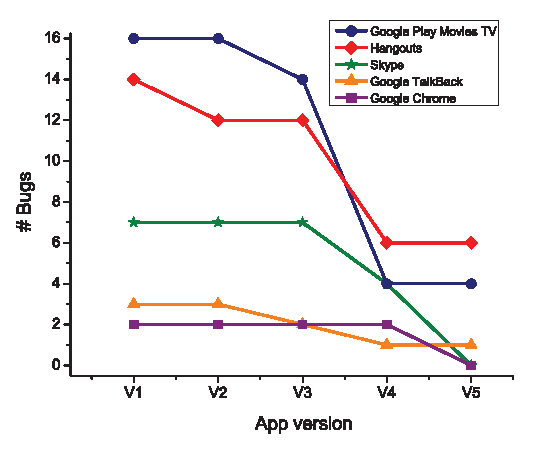
\includegraphics[scale=0.35]{bugs-vs-versions.eps}
 \caption{The number of services usage inefficiency bugs decreases in newer versions.}
\label{fig_bugsvsversions}
\end{figure}


\section{Related Work}\label{relatedwork}
Our research is related to work on GUI testing, service analysis and testing,
and performance (energy) testing of Android apps. In the following, we review
some existing work on these topics.

\textbf{GUI testing}. Most existing testing approaches for Android apps focus on GUI testing. According to the exploration strategies employed, Choudhary et al.~\cite{ChoudharyGO15} summarize three main categories of testing approaches: \textit{random testing}~\cite{monkey,HuN11,MachiryTN13,SongQH17}, \textit{model-based testing}~\cite{GUIRipping,grey-box,ChoiNS13,a3e,SuMCWYYPLS17}, and \textit{advanced testing}~\cite{AnandNHY12,JensenPM13,EvoDroid,MaoHJ16}. Although \textsf{Monkey}~\cite{monkey} is among the first generation techniques for Android testing, compared with many follow-up approaches, it still shows good performance and advantages in app testing~\cite{ChoudharyGO15}. \textsf{Dynodroid}~\cite{MachiryTN13} improves \textsf{Monkey} by reducing the possibility of generating redundant events. It achieves this by monitoring the reaction of an app upon each event and basing on the reaction to generate the next event. Recently, \textsf{EHBDroid}~\cite{SongQH17} is presented to first instrument the invocations of event callbacks in each activity and then directly trigger the callbacks in a random order. This approach is more efficient as it bypasses the GUI for test input generation. Since random testing may generate redundant events, several model-based testing approaches are proposed~\cite{AmalfitanoFT11,GUIRipping,grey-box,ChoiNS13,a3e,BaekB16,SuMCWYYPLS17}. These approaches first obtain a model of the app GUI, and then generate test input according to the model. While most of them utilize program analysis techniques to obtain the model, machine learning is used in~\cite{ChoiNS13} to learn the model. The third category approaches leverage advanced techniques to efficiently generate effective event sequences for app testing\cite{AnandNHY12,JensenPM13,EvoDroid,MaoHJ16}. For example,  \textsf{ACTEve}~\cite{AnandNHY12} uses symbolic execution and \textsf{EvoDroid}~\cite{EvoDroid} employs evolutionary algorithm to generate event sequences. \textsf{Sapienz}~\cite{MaoHJ16} formulates the event sequence generation as a multiple-objective optimization problem and employs search-based algorithm to generate the shortest event sequences that can maximize the code coverage and bug exposure.

\textbf{Service analysis and testing}. A number of work concentrates on the
security vulnerabilities (e.g., denial of service, single point failure) of
Android system services~\cite{ReavesBGABCDHKS16,HuangZ0015,WangZL16,FengS16,AbualolaAKOM16,LuoZCCLLGYXL17}.
In terms of app services, Khanmohammadi et al.~\cite{KhRH15} find that malware
may use background services to perform malicious operations with no communication with
the other components of the app.
They propose to use classification algorithms to differentiate normal and
malicious apps based on the service features related to their lifecycle. In
contrast to GUI testing for activities, background service testing gains little
attention.  Lee et al. present a system facility for analyzing energy consumption of Android system services~\cite{LeeJCC15}. \textsf{Snowdrop}~\cite{ZhangLLC17} is among the first to
automatically and systematically testing background services in apps. Since not
all \textit{Intent} messages can be directly derived from the app bytecode,
\textsf{Snowdrop} infers field values based on a heuristic that leverages the
similarity in how developers name variables. This approach can find general bugs
(functional bugs that lead to app crashes) in services, but may meet
difficulties in detecting service usage inefficiency bugs targeted in our work.
A dynamic analysis tool~\textsf{LESDroid}~\cite{ma2018} is presented to find
exported service leaks, whereas \textsf{ServDroid} is a static analysis tool and
is more general, which cannot only find both private and exported service leaks
but also detect the other three kinds of service usage inefficiency bugs.

\textbf{Performance testing}. Non-functional or performance bugs in apps are
also important for user experience. Liu et al.~\cite{LiuXC14} conduct an
empirical study on 29 popular Android apps and find three types of performance
bugs: GUI lagging, energy leak, and memory bloat. They also summarize common
performance bug patterns (including lengthy operations in main threads, wasted
computation for invisible GUI, and frequently invoked heavy-weight callbacks)
and propose method to detect them. Since energy is a major concern in app
performance and green software
engineering~\cite{PangHAH16,HoqueSKXT16,MBZSJSPC16,0036990}, energy bugs and the
corresponding detection and testing solutions draw increasing attention~\cite{QianWGMSS11,PathakJHM12,VasquezBBOPP14,GuoZYZZ13,BanerjeeC0R14,LiuXCL14,BehrouzSBM16,WuYR16,JabbarvandM17}.
Pathak et al. study app energy bugs which arise from mishandling power control APIs~\cite{PathakJHM12}.  Based on a hardware power monitor, V{\'{a}}squez et al. mine and
analyze energy-greedy API usage patterns that correspond to suboptimal usage or choice of APIs. Chen et al. show that apps can drain battery even while running in background, and they present a system that can suppress background activities that are not required to the user experience~\cite{ChenJDHGV15}. However, these researches do not consider service usage anti-patterns presented in this paper. It is worth mentioning that energy bugs are highly relevant to resource
leaks~\cite{GuoZYZZ13,BanerjeeC0R14,LiuXCL14,WuYR16}. Banerjee et
al.~\cite{BanerjeeC0R14,BanerjeeCBR18} present a testing framework to detect energy bugs and
energy hotspots in apps based on the measurement of the power consumption through a power meter.
Although the framework also considers service leak bugs, the test oracle based
on the power consumption is expensive and time-consuming.
To reduce the cost of testing, Jabbarvand et al.~\cite{BehrouzSBM16} propose an
approach to minimize the energy-aware test-suite. Wu et
al.~\cite{WuYR16} present a static analysis approach to detecting GUI-related energy-drain
bugs, whereas our approach aims to detect service usage inefficiency bugs.

\section{Conclusions}\label{conclusion}
It is extremely challenging for testing techniques to reveal service usage
inefficiencies in apps, because such latent bugs do not exhibit
immediate bug symptoms such as crashes.
We have conducted an in-depth study of Android services, and presented four
anti-patterns that lead to service usage inefficiency bugs and a static
analysis approach to automatically detect all them. To our knowledge,
this work is among the first to detect service performance bugs using static
analysis. We also implemented an open-source tool {\sf ServDroid} and conducted
an empirical evaluation on 45 real-world Android apps. The empirical results
demonstrate that service usage inefficiency bugs are severe in practice and they
have a significant negative impact on energy consumption.

To complement the static analysis, we plan to present dynamic analysis techniques to detect service usage inefficiency bugs.

%\section*{Acknowledgments}
%This work was supported in part by the National Key R\&D Program of China under Grant No. 2017YFB1001801, the National Natural Science Foundation of China under Grant No. 61761136003, the Natural Science Foundation of Jiangsu Province under Grant No. BK20171427.

\bibliographystyle{ACM-Reference-Format}
\bibliography{ref}

\end{document}
